\documentclass[11pt]{article}
\usepackage[letterpaper,margin=.72in]{geometry}
\usepackage[T1]{fontenc}
\usepackage{lmodern,microtype,graphicx,booktabs,amsmath,hyperref}
\hypersetup{colorlinks=true,urlcolor=blue,pdfauthor={James N. Jean IV},pdftitle={Airport-zone pickup capacity under asymmetric scenario costs}}
\setlength{\parindent}{0 pt}\setlength{\parskip}{6 pt}\renewcommand{\arraystretch}{1.1}
\begin{document}
{\Large\bfseries Airport-zone pickup capacity under asymmetric scenario costs}\par
James N. Jean IV\hfill 29 October 2026\par
\textit{Independent study 04. Not peer reviewed.}
\section*{Decision brief}
Should a median or a higher count quantile guide an airport pickup-capacity scenario? This comparison uses 2024 published yellow-taxi records at JFK and LaGuardia taxi zones. Its target is recorded meter engagements, not latent requests, unique deduplicated trips, passenger queues or waiting time.

\textbf{Conditional finding.} The frozen 75th-percentile policy has 4.5\% lower held modeled cost than the median under a hypothetical 250-services-per-zone-hour cap and underage/excess costs 3:1. Cost totals are 633,760 versus 663,611 units across 4,368 held zone-hours. Raw-count MAE is worse: 48.727 versus 42.022. On the two fixed holiday stress dates, its cost is 15.1\% higher: 8,153 versus 7,086 units. All planned comparisons and these failures are retained.

\textbf{Evidence needed before action.} Obtain timestamped dispatch telemetry, vehicle service cycles, actual supply/costs and queue outcomes before a prospective test. Public historical records do not verify real-time availability. The present comparison assumes immediate prior-day counts and one service per vehicle-hour, without inter-hour carryover. It establishes neither operational readiness nor realized savings.
\begin{center}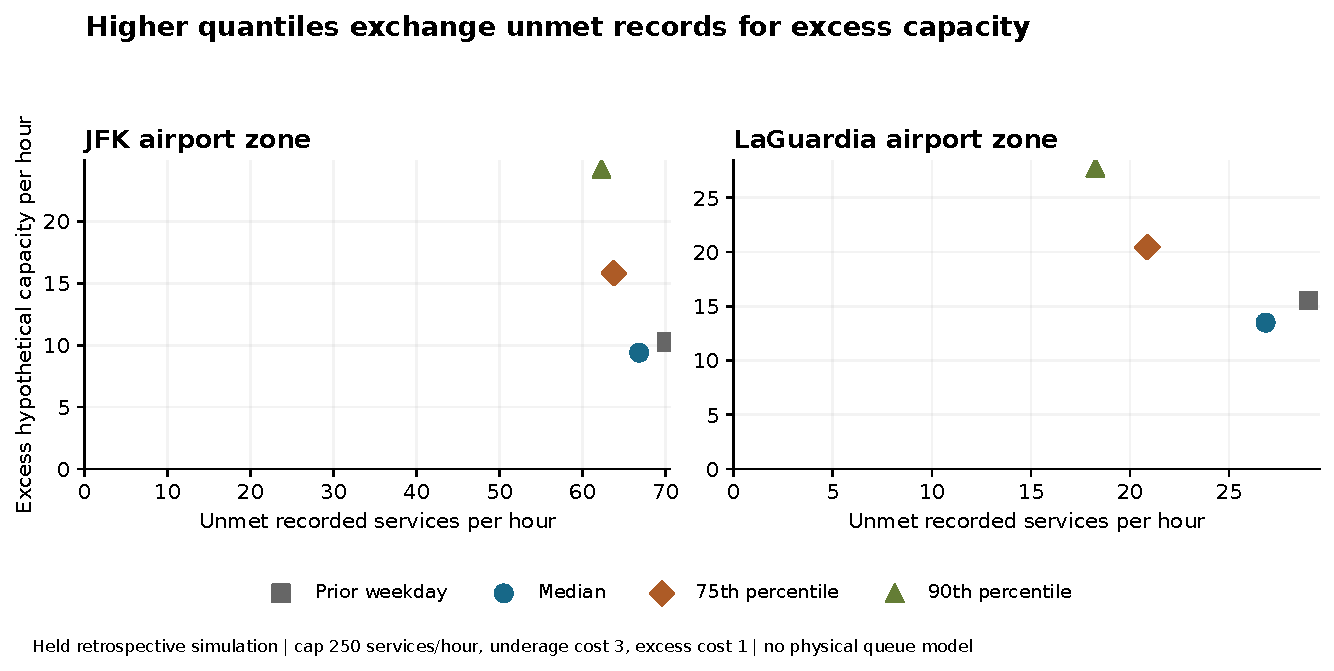
\includegraphics[width=\linewidth]{images/capacity_tradeoff.pdf}\end{center}
\small Figure 1. Complete held primary airport tradeoffs. Higher quantiles reduce unmet recorded services while increasing excess hypothetical capacity. Counts are published records; cost assumptions and the absence of a physical queue model limit interpretation.\normalsize
\newpage
\section*{1. Fixed source, timing and policy design}
The official NYC Open Data 2024 Yellow Taxi Trip Data (rwwi-khbc) identifies pickup time as meter engagement and pickup location as the TLC taxi zone [1--3]. Official lookup facts identify 132 as JFK Airport and 138 as LaGuardia Airport. TLC disclaims source accuracy; these records come from technology providers. The historical dataset was published in 2026, and TLC generally releases monthly records after collection. Exact historical vintages and dispatcher telemetry are unavailable. Past-only date indices are checked under an \textbf{idealized prior-day availability assumption}; no genuine prospective availability clearance is claimed.

Only coarse airport/day/hour count queries, independent daily/monthly controls and source-quality diagnostics were retrieved. The captured scope has 3,285,485 airport records and 17,568 nominal civil grid cells, including 578 absent groups filled with zero published records. That does not imply zero latent demand or complete reporting. Before/after metadata revisions match: row update 1787344789 and view modification 1787345062. All source queries and response hashes are retained. Independent SQL grid/control reconciliation performs 106,538 checks.

Floating local timestamps do not distinguish repeated DST hours. Entire March 10 and November 3 dates are flagged and excluded from histories/targets, retaining 20,054 source records outside the model. No UTC-duration claim follows. Initial history has 8,688 zone-hour bins; July--September validation has 4,416; October--December held targets have 4,368. No low counts, outliers or holidays are silently removed.

For each zone, civil hour and target day, history uses dates in $[t-W,t)$, with $W\in\{28,56,84\}$ days. Calendar groups match weekday/hour or weekday-versus-weekend/hour. Quantiles are 1/2, 3/4 and 9/10, using order rank $\lceil qn\rceil$ without interpolation, with at least 3 history observations. The baseline takes the most recent available same-weekday/hour count within 28 days, skipping the two excluded dates. All 18 grid configurations and the baseline retain every validation prediction, history size/boundary and per-policy runtime. No regression estimator or stochastic training is used.

For recorded count $d$, proposed count $p$ and hypothetical cap $K$, allocate $a=\min(p,K)$, unmet $u=\max(d-a,0)$ and excess $e=\max(a-d,0)$. Cost is $c_u u+e$. Caps are 100, 250 and 500 services/hour; underage costs are 1, 3 and 9, with excess cost 1. These are untuned scenario assumptions, not measured fleets or money. Primary selection uses pooled validation cost at $K=250,c_u=3$. Exact ties prefer daytype/hour, shorter history, then smaller quantile. Each quantile selects an 84-day weekday/hour policy; the 75th percentile wins the same declared comparison.

Protocol commit 089f464 precedes count retrieval. Twenty-one canonical dependencies and selection bytes from 95c4aca are publicly frozen in 8a11b68 before held analytical outcomes. Source inputs and quality were visible without blinding. Prior held counts may enter later histories under the same explicit immediate-availability assumption; no future target date enters a history. The three quantile comparators and baseline are frozen before evaluating all nine cap/cost settings.
\newpage
\section*{2. Complete primary held comparison}
Every airport has 2,184 held target hours; pooled summaries have 4,368. MAE below is uncapped absolute record-count error per zone-hour. Unmet/excess are hypothetical service/capacity totals. Cost/hour uses the fixed 3:1 scenario, not currency. Exact counts and rational rates remain in the exported results.
\begin{center}\small\setlength{\tabcolsep}{4 pt}
\begin{tabular}{llrrrr}\toprule
Scope & Policy & Raw MAE & Unmet & Excess & Cost/hour\\\midrule
JFK & Prior weekday & 51.609 & 153,222 & 22,392 & 220.723 \\
JFK & Median & 44.854 & 145,923 & 20,530 & 209.844 \\
JFK & 75th percentile & 55.088 & 139,265 & 34,564 & 207.124 \\
JFK & 90th percentile & 73.422 & 136,005 & 52,887 & 211.036 \\
LGA & Prior weekday & 46.962 & 63,353 & 33,895 & 102.543 \\
LGA & Median & 39.190 & 58,625 & 29,437 & 94.007 \\
LGA & 75th percentile & 42.366 & 45,591 & 44,628 & 83.059 \\
LGA & 90th percentile & 53.683 & 39,863 & 60,569 & 82.490 \\
Pooled & Prior weekday & 49.285 & 216,575 & 56,287 & 161.633 \\
Pooled & Median & 42.022 & 204,548 & 49,967 & 151.926 \\
Pooled & 75th percentile & 48.727 & 184,856 & 79,192 & 145.092 \\
Pooled & 90th percentile & 63.552 & 175,868 & 113,456 & 146.763 \\
\bottomrule\end{tabular}\end{center}
The 75th policy reduces pooled unmet recorded services from 204,548 to 184,856 but raises excess capacity from 49,967 to 79,192. Its 29,851-unit primary cost reduction is conditional on the 3:1 coefficient and cap. The 90th policy has the lowest primary cost at LaGuardia, while 75th wins pooled and at JFK; no subgroup policy is reselected from held results.
\begin{center}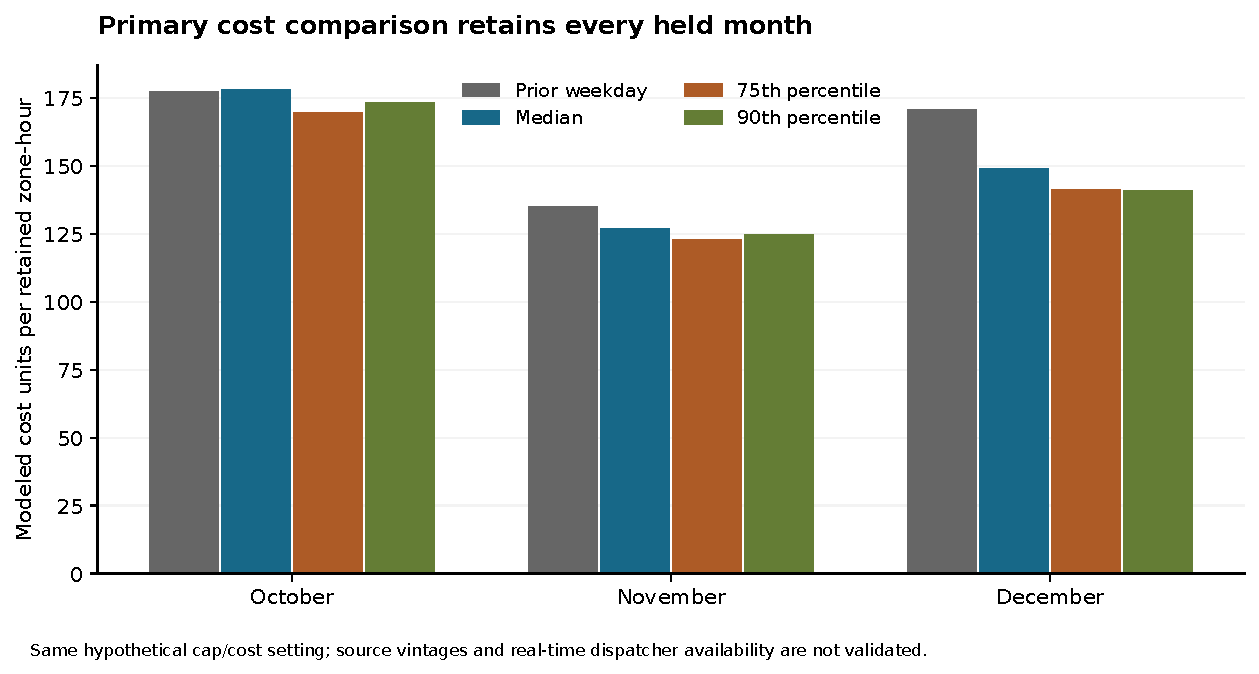
\includegraphics[width=.97\linewidth]{images/monthly_costs.pdf}\end{center}
\small Figure 2. Every held month is retained at the primary scenario. Pooled 75th-minus-median cost differences are $-12,409$ in October, $-6,080$ in November and $-11,362$ in December. All three leave-one-held-month-out mean differences also remain negative; their finite range is a temporal sensitivity, not a confidence interval or future-coverage guarantee.\normalsize
\newpage
\section*{3. Cost assumptions and retained stress failures}
\begin{center}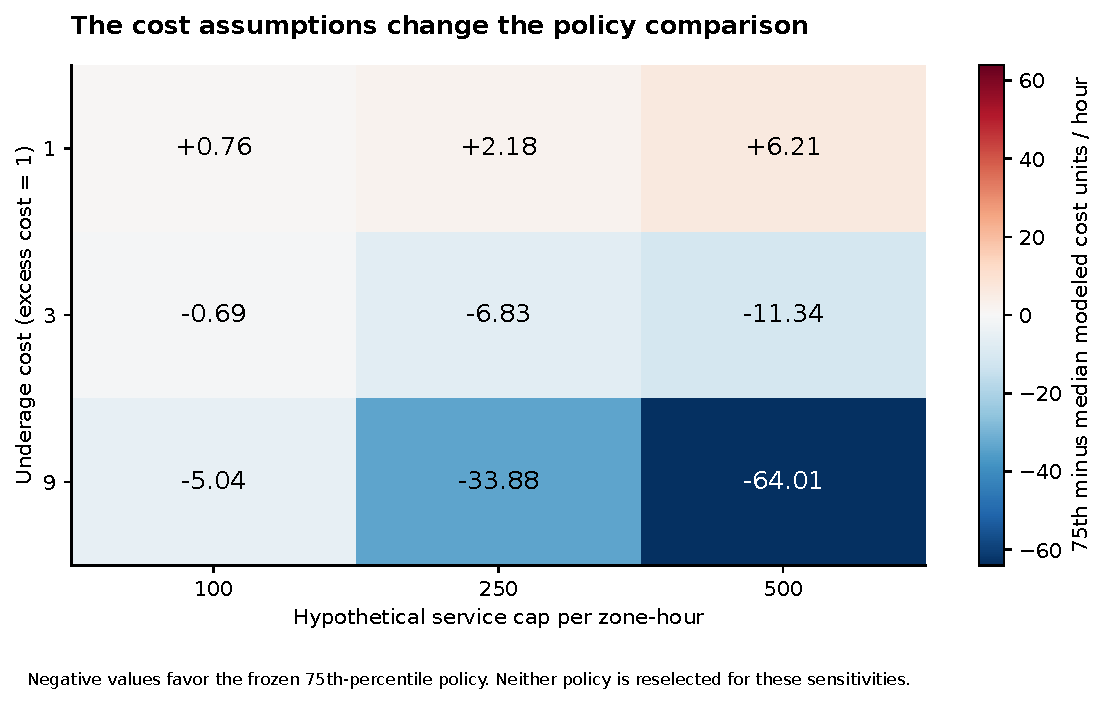
\includegraphics[width=.96\linewidth]{images/cost_assumptions.pdf}\end{center}
\small Figure 3. Frozen 75th-minus-median cost per held zone-hour for every declared cap/cost setting. Negative values favor 75th; positive values favor the median. At equal underage/excess cost, 75th costs more at all three caps. Policies are not reselected for the sensitivity outcomes.\normalsize

Thanksgiving (November 28) and Christmas (December 25) are the fixed OPM 2024 stress dates [4], totaling 96 zone-hours. They are two named days, not a representative holiday sample or a causal holiday experiment. Higher-quantile policies incur more excess hypothetical capacity on these days.
\begin{center}\small
\begin{tabular}{lrrr}\toprule
Policy & Unmet & Excess & Modeled cost\\\midrule
Prior weekday & 192 & 6,019 & 6,595 \\
Median & 189 & 6,519 & 7,086 \\
75th percentile & 172 & 7,637 & 8,153 \\
90th percentile & 160 & 8,245 & 8,725 \\
\bottomrule\end{tabular}\end{center}
The 75th policy costs 1,067 units more than the median on these stress dates, or 15.1\% after rounding. This failure is retained despite lower full-period primary cost. Its raw-count exceedance frequency is also an empirical frequency, not a probability-calibration guarantee. Capping changes shortage frequency, so capped shortages must not be conflated with raw quantile exceedances. Complete airport/month, stress-date, joint-stress and scenario summaries are exported.

Twelve fixtures cover rank endpoints, ties, capacity arithmetic, past-only calendars, insufficient history, baseline fallback and selection ties. An independent checker does not import forecasting, selection or metric helpers. SQL window ranks reconstruct every history/order statistic; independent integer/rational calculations reconstruct all scenario totals, selections, exact boundaries and temporal sensitivities. Square-root RMSE checks use absolute tolerance $10^{-12}$; categorical, count and rational checks are exact.
\newpage
\section*{4. Reproduction, limitations and evidence status}
Independent reconstruction checks 83,904 validation predictions, 17,472 held predictions and 2,592 scenario metric rows, totaling 956,489 numeric/history checks including RMSE tolerances. The isolated replay matches 1,177,457 CSV fields and selection documents and verifies 21 protected dependencies. Per-policy original timings are retained; variable replay timings are excluded from deterministic identity. The three original figures have 37 actual artist-value checks and 9 heatmap annotation/contrast checks. Visual review is separate and does not establish accessibility conformance.

\textbf{Source minimization correction.} The initial all-city quality query included exact minimum/maximum timestamp extrema. That response remains private and is excluded from public output. Before publication, corrected diagnostics use day-only extrema; count totals and source revisions match. Individual trip rows, IDs, fares, dropoffs and passenger fields were not downloaded. The initial query and correction are documented without publishing extrema. No count, model, selection or held outcome changed.

\textbf{Material limits.} Historical public files are delayed and may be corrected. The study cannot verify data vintages available at a 2024 dispatch origin. Meter engagements omit unserved requests and do not measure latent demand, passenger arrival time, queue waits or taxi availability. The simulation assumes one service per vehicle-hour, no return/repositioning time, fixed caps, fixed scenario costs and no inter-hour carryover. Those assumptions are not empirically calibrated. No live dispatch, causal benefit, money saving, complete reporting, predictive deployment or exhaustive novelty claim follows. The held period is only three months at two zones. Finite month/stress sensitivity is not statistical generalization.

\textbf{Reproduction} from the repository root:
\begin{quote}\small\ttfamily
python -m pip install -r requirements.txt\par
python -m unittest discover -s tests -v\par
python src/check\_reproduction.py\par
python src/verify\_figures.py\par
python src/verify\_paper.py\par
python src/verify\_public\_package.py
\end{quote}
Public replay uses the captured coarse aggregate snapshot rather than silently requesting a later source version. Release additionally requires scoped canonical-blob/privacy checks, exact-head Linux replay and matching merged tree/annotated tag. The manuscript is independent program work, not peer reviewed. Formal-publication projects, including Azure optimization, remain private.

\section*{References}
\small
[1] NYC Taxi and Limousine Commission. \href{https://www.nyc.gov/site/tlc/about/tlc-trip-record-data.page}{TLC Trip Record Data}; source/accuracy and publication-delay notes. Accessed 29 October 2026.\par
[2] NYC Open Data/TLC. \href{https://data.cityofnewyork.us/Transportation/2024-Yellow-Taxi-Trip-Data/rwwi-khbc}{2024 Yellow Taxi Trip Data}, published 2026; exact metadata and count-query hashes in the source manifest.\par
[3] TLC. \href{https://www.nyc.gov/assets/tlc/downloads/pdf/data_dictionary_trip_records_yellow.pdf}{Yellow Taxi Data Dictionary}; official-linked zone lookup at \href{https://d37ci6vzurychx.cloudfront.net/misc/taxi_zone_lookup.csv}{TLC zone facts}. Full documents/artwork excluded.\par
[4] U.S. Office of Personnel Management. \href{https://www.opm.gov/policy-data-oversight/pay-leave/federal-holidays/}{Federal Holidays, 2024 schedule}. Named stress dates only.
\end{document}
